%----------------------------------------------------------------------------------------
%	Hardware
%----------------------------------------------------------------------------------------

\chapter{Hardware Components}

\section{Final Design}

The hardware consists of: circuitry to connect weight sensors and output a signal from them; power conditioning circuitry; a microcontroller; and LEDs and buttons for user interaction. The role of the hardware is to provide power to the scale, accurately take measurements of weight to send to the microcontroller (which contains the embedded software), and display the real-time weight on the scale to the user. Only functionalities deemed essential to the scale’s accuracy and usability have been included to reduce unnecessary component and natural materials usage which are taonga. A block diagram of the hardware is in Figure \ref{fig:hardware-block}. The detailed hardware schematic is in Figure \ref{fig:schematic} with the printed circuit board (PCB) in Figure \ref{fig:hardware-pcb}. The cost of one hardware prototype is \$30.61.

\begin{figure}[!ht]
	\centering
	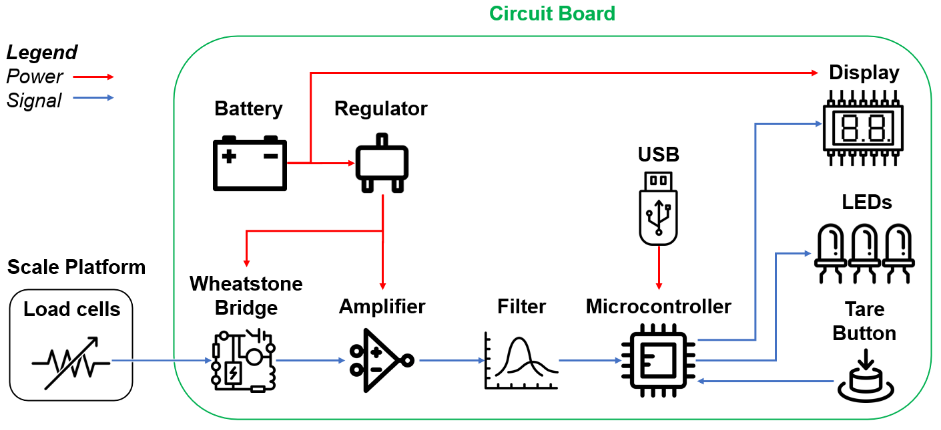
\includegraphics[scale=0.5]{hardware-block.png}
	\caption{Hardware block diagram.}
	\label{fig:hardware-block}
\end{figure}

To detect weight on the scale, four load cells are used. They react to weight by having an electrical resistance that changes linearly when weight is applied to them. They are used to accurately measure weight by connecting them into a Wheatstone bridge circuit. With one load cell in each corner of the scale, they accurately sense the weight of any dog on it, even if the dog isn’t centred. This reduces the stress on SPCA staff as it can be very difficult to make a dog sit in the exact centre of a scale. A Wheatstone bridge is used because it requires no additional components and has high resolution output for higher accuracy than other topologies.

The signal from the Wheatstone bridge is small and thus is amplified before being sent to the microcontroller. A larger signal will have greater digital resolution, allowing for greater accuracy of measurement which is important for the scale so that animals in the SPCA’s care can get proper treatment. To amplify the signal, an instrumentation amplifier is used because it is robust against common mode electrical noise which can corrupt the signal’s accuracy. Common mode noise is the electrical noise (random high frequency signals) that exists in both signals of the amplifier’s inputs. Even if resistors in the amplifier circuit aren’t the exact value they need to be, the instrumentation amplifier will still be able to reject the noise well compared to alternatives.

The LM324 operational amplifier used for the instrumentation amplifier, chosen as a low cost and common amplifier that is unlikely to reach obsolescence, with a standard footprint for simple replacement. An amplification of 1600 is chosen to maximise the linear 0.02V-1.8V output range of the LM324 (with a 3.3V supply), ensuring a linear relationship that is easy to process in the embedded software. However, to overcome the lower output limit, a 0.1V offset is added from a voltage divider and buffer which is reliable and cheap. By adding this offset, it ensures that even small changes in weight less than 0.5kg can be accurately detected and measured, rather than the signal not being able to be output if less than 0.1V, which it could be at low weights. Future changes to the gain or offset are as simple as replacing a single resistor, thus the design is robust to changes in load cell selection or the weight detection range of the scale.

Before being sent to the microcontroller, the signal goes through a resistor-capacitor (RC) filter to remove differential mode noise from the signal. Differential mode noise is the noise that exists only in individual signals, rather than multiple signals like common mode noise. However, both types of noise can corrupt the signal. Filtering the differential mode noise ensures the signal is as noise-free as possible before it is sent to the microcontroller for processing in the embedded software.

To power the circuitry, the hardware is supplied with 6V from four AA batteries. To regulate the voltage of the batteries which inherently decrease over time, a 3.3V linear regulator is used as a cost effective solution. Voltage regulation is important to ensure the output signal representing weight that goes to the microcontroller does not drift with the battery’s voltage. A linear regulator is less efficient than a switched mode regulator, however it does not produce electromagnetic interference; simplifying future costly compliance certification processes.

To interact with the user, the scale has several features. The scale has LEDs to indicate to a user: when the scale is powered; when the scale has been zeroed; and when a measurement has been taken. The scale also has a four digit display to show real-time weight measurements in kg, allowing the scale to be used in an analog manner, rather than always requiring a phone or laptop. It also has a tare button to zero it.

\begin{figure}[!ht]
	\centering
	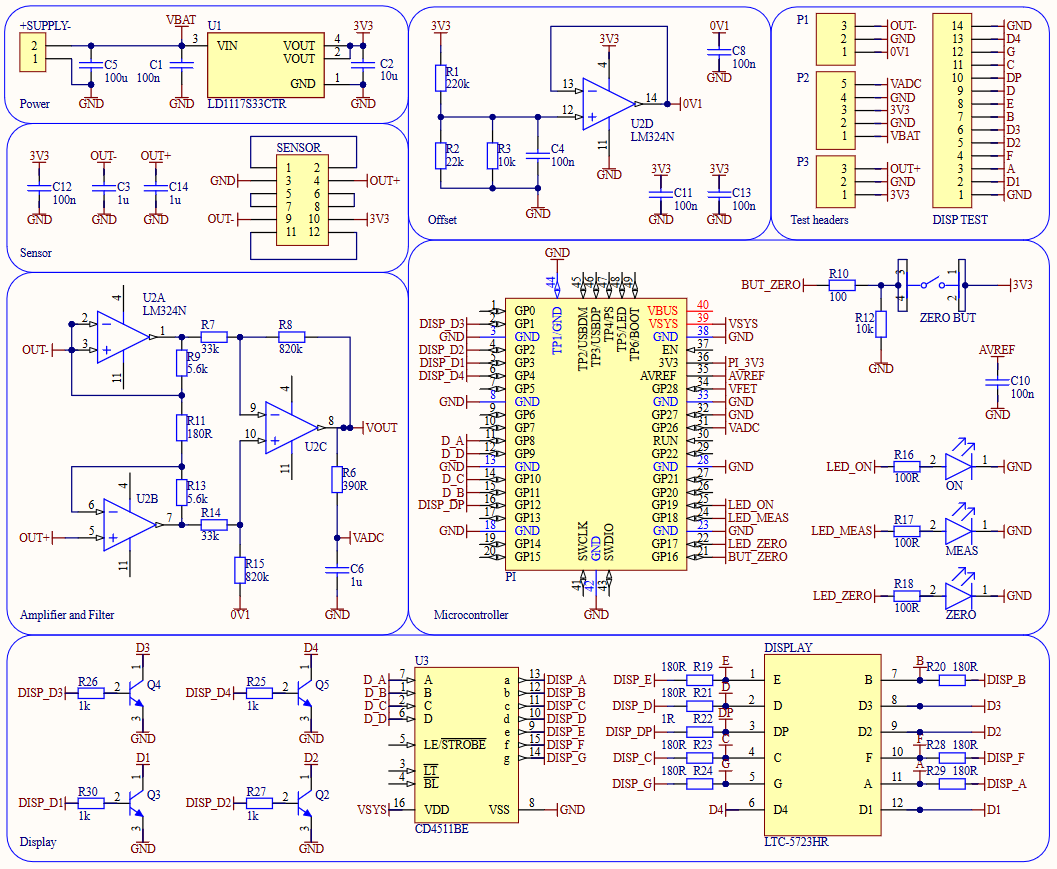
\includegraphics[scale=0.55]{hardware-schem.png}
	\caption{Detailed hardware schematic.}
	\label{fig:schematic}
\end{figure}

\begin{figure}[!ht]
	\centering
	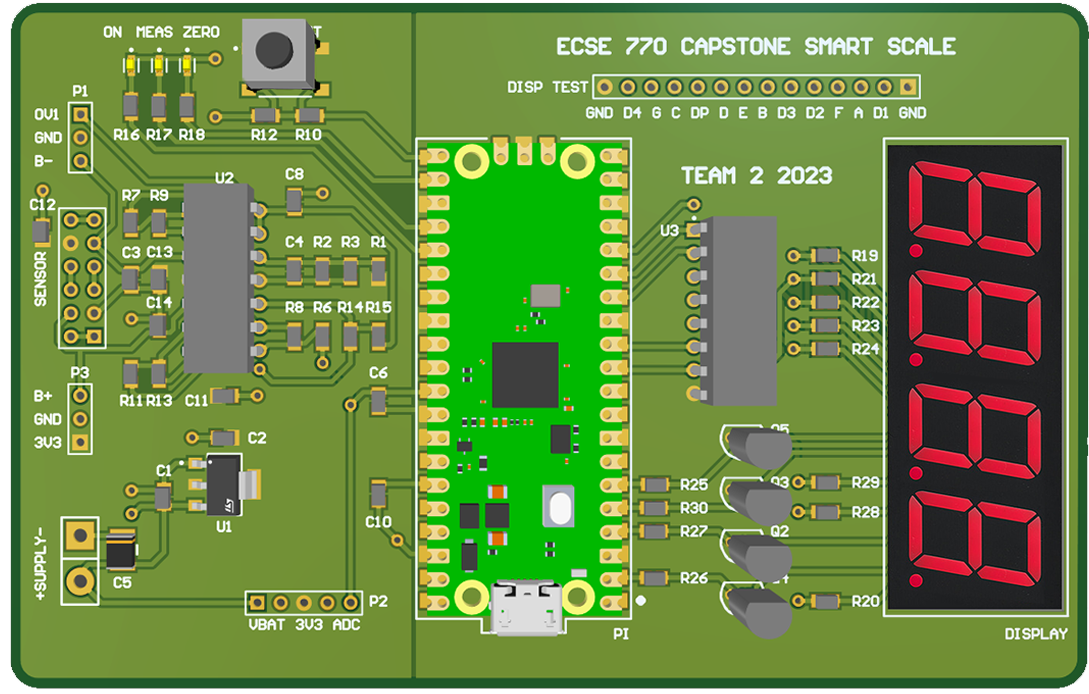
\includegraphics[scale=0.5]{hardware-pcb.png}
	\caption{Hardware printed circuit board (PCB).}
	\label{fig:hardware-pcb}
\end{figure}

The PCB in Figure \ref{fig:hardware-pcb} incorporates the hardware into a compact board. It separates components into functional groups to reduce electrical noise in the weight measurement signal that goes to the microcontroller, for increased accuracy. Surface mount components are used because they are small which requires less physical resources than through-hole components, making the design more environmentally friendly, and they are cheaper too. No uncommon components are chosen. Thus, in the case of obsolescence, components should be easily replaceable. Further, components with long lifetimes were chosen to maximise the lifespan of the scale. For example, electrolytic capacitors were not used in the design as they are often the first point of failure of an electronic device.

\section{Validation}

The technical requirements of the hardware are in Table \ref{tab:hardware-requirements}. The performance of the scale’s hardware is validated in Table \ref{tab:hardware-testing} against the required specifications. They are met besides 5 and 7, whose testing was not conducted. For future development, testing is suggested to observe the operating temperature to meet specification 5. Certification is required to meet specification 7. The resolution accuracy of the weight measurement (specification 3) will be discussed in the Embedded Software section where the output voltage from the hardware is processed into the weight of a dog in kg.

\begin{table}[!ht]
	\centering
	\caption{Hardware specifications.}
	\begin{tabular}{lll}
		\hline
		\multicolumn{1}{c}{Number} & \multicolumn{1}{c}{Parameter} & \multicolumn{1}{c}{Value} \\
		\hline
		1                          & Supply Voltage                & 4 AA batteries            \\
		2                          & Weight Range                  & 0.5 to 25 kg              \\
		3                          & Weight Accuracy               & 0.5 kg                    \\
		4                          & Output Voltage Range          & 0 to 3V                   \\
		5                          & Operating Temperature         & 0 to 40°C                 \\
		6                          & Display                       & Measure success, tare     \\
		7                          & Compliance                    & AS/NZS 5377, RoHS, WEEE  
	\end{tabular}
	\label{tab:hardware-requirements}
\end{table}

\begin{table}[!ht]
	\centering
	
	\caption{Hardware testing of specifications.}
	\begin{tabular}{cllll}
		\hline
		Specification & Test & Expected Result & Actual Result/s & Pass/Fail\\
		\hline
		1 & Regulator supply voltage & 3.3 V & 3.3 0V & Pass\\
		2 & \multicolumn{4}{l}{Shown in Figure \ref{fig:results}.}\\
		3 & \multicolumn{4}{l}{Discussed in Embedded Software.}\\
		4 & Output voltage with 0 kg on scale & Minimum 0.1 V  & 0.17 V & Pass\\
		4 & Output voltage with 25 kg on scale & Maximum 1.8 V  & 1.69 V & Pass\\
		5 & \multicolumn{4}{l}{Untested.}\\
		6 & Scale tared & Display shows 0 kg  & 0.03 kg
		& Pass\\
		6 & Weight measurement is saved & LED and display blink  & Expected 	 & Pass\\
		7 & \multicolumn{4}{l}{Untested. Discussed in Compliance.}\\
	\end{tabular}
	\label{tab:hardware-testing}
\end{table}

\begin{figure}[!ht]
	\centering
	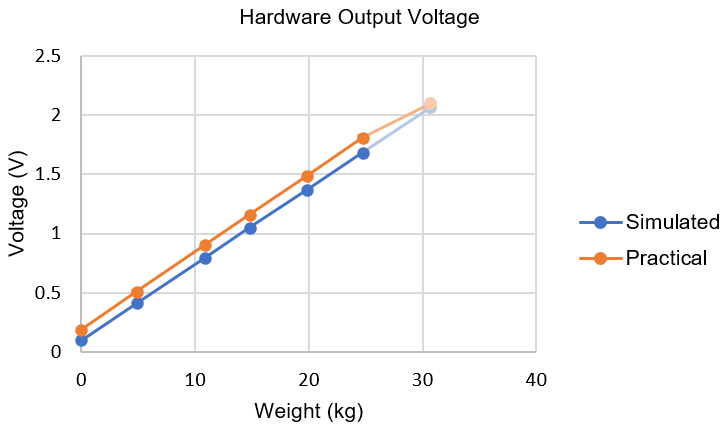
\includegraphics[scale=0.5]{hardware-results.png}
	\caption{LTSpice and practical hardware testing results.}
	\label{fig:results}
\end{figure}


The output signal was also measured with different weights on the scale to validate its linearity, with results in Figure \ref{fig:results}. Linearity is important for simple processing in the microcontroller with more accurate measurement of weights. The signal varies linearly as expected within the range 0-25 kg. There is saturation of the signal after 25kg where the relationship begins to become non-linear. The amplifier could be modified to achieve a greater linear measurement range of dog weights if required by the SPCA. Repeatability testing showed a maximum deviation of 1\%. This high precision indicates the scale can reliably measure weights for the SPCA. High repeatability is also essential for mass production to ensure that each unit produces the same results. 

\section{Compliance}

As per specification 7 in Table \ref{tab:hardware-requirements}, the scale must comply with RoHS, WEEE, and AS/NZS 5377. These directives and standards outline requirements related to the use of hazardous materials in electronics and the disposal of electronic waste (e-waste). They are compulsory to comply with for mass production of the scale. Complying with these standards will also help to create a more sustainable and robust design.

RoHS outlines the restriction of 10 materials in electrical equipment to reduce risk to humans and the environment. For the scale to comply with RoHS, it should only use components that are RoHS compliant and do not contain other restricted substances. The scale must be sent for time-consuming and expensive verification before it can achieve compliance.

WEEE outlines what should happen to electrical and electronic waste to reduce landfill waste. For the scale to comply with WEEE, several steps must be taken. Firstly, the project must be registered with the required national authorities who will require documentation. The documentation should detail what should happen to the scale at the end of life including: the locations of appropriate e-waste disposal centres; disassembly instructions; and what components can be reused or refurbished. All documentation should be revised annually. The scale itself should be developed for recycling and end-of-life. For example, it should use standard connectors that are easy to disassemble with common tools and connectors. Further, components and materials should be labelled so it is easy to sort them at the e-waste centre at the scale’s end-of-life. Additionally, the scale itself could use recycled materials. For example, mechanical enclosures of existing scales could be used and fitted with the smart scale’s hardware, reducing the use of new materials. By considering and implementing these design choices, the design will be better suited to recycling and refurbishment, creating a more sustainable product.

AS/NZS 5377 outlines requirements for storing, transporting, and disposing of electrical equipment and waste with regard to the environment, sustainability, and human health. For the scale to achieve compliance with AS/NZS 5377, at the end of its life, it should be taken to a designated e-waste facility that is AS/NZS 5377 certified, where it will be disassembled as per the documentation written to meet WEEE. When taken to an e-waste facility, the transportation journey should be as short as possible. Further, to reduce the carbon footprint of the scale, it should be developed to be durable to last as long as possible. To achieve this, the scale should use components and materials that have long lifetimes, and it should operate only in the expected conditions. By increasing the lifespan of the scale, it also reduces the potential landfill waste it could cause. To further increase its lifespan, the scale could be developed to be modular such that a user could replace modules without much technical knowledge or debugging. Modules could include signal processing, microcontroller, LED display, and power. Each module would have inbuilt fault detection and indicator LEDs to easily know if a module is faulty. If a module was faulty, documentation could be provided to the user to do replacements of modules. Thus the scale could be self-maintained rather than disposed of or requiring complex repairs. This would allow the scale’s hardware to last longer, even once components need replacing. The scale should also minimise the power consumed during operation. This change could be implemented by turning the regulator off after a timeout period of the scale not being used. This design is more user-friendly than having an on and off button, and does not rely on a user to turn the scale off, making it easier to use. Turning the regulator off will also significantly reduce the power consumption of the scale, allowing it to require less energy, and decrease the frequency of battery replacements. Currently, the scale saves power by implementing a sleep feature in the Embedded Software. With any changes made, documentation should be written to detail the steps taken to minimise the scale’s carbon footprint. Finally, quality assurance testing should be completed to validate the scale’s lifespan, which should also be documented.
Overall, suggestions are made to achieve compliance with RoHS, WEEE, and AS/NZS 5377. Compliance must be fulfilled before the scale can be brought to production.
